\documentclass[border={0.1cm 0.1cm 0.1cm 0.1cm}]{standalone}  %E,S,W,N

\usepackage{amssymb}
\usepackage{amsmath}
\usepackage{tikz}
\usetikzlibrary{shapes} %for node shapes
%\usetikzlibrary{calc}	%for centerarc

\begin{document}
	
	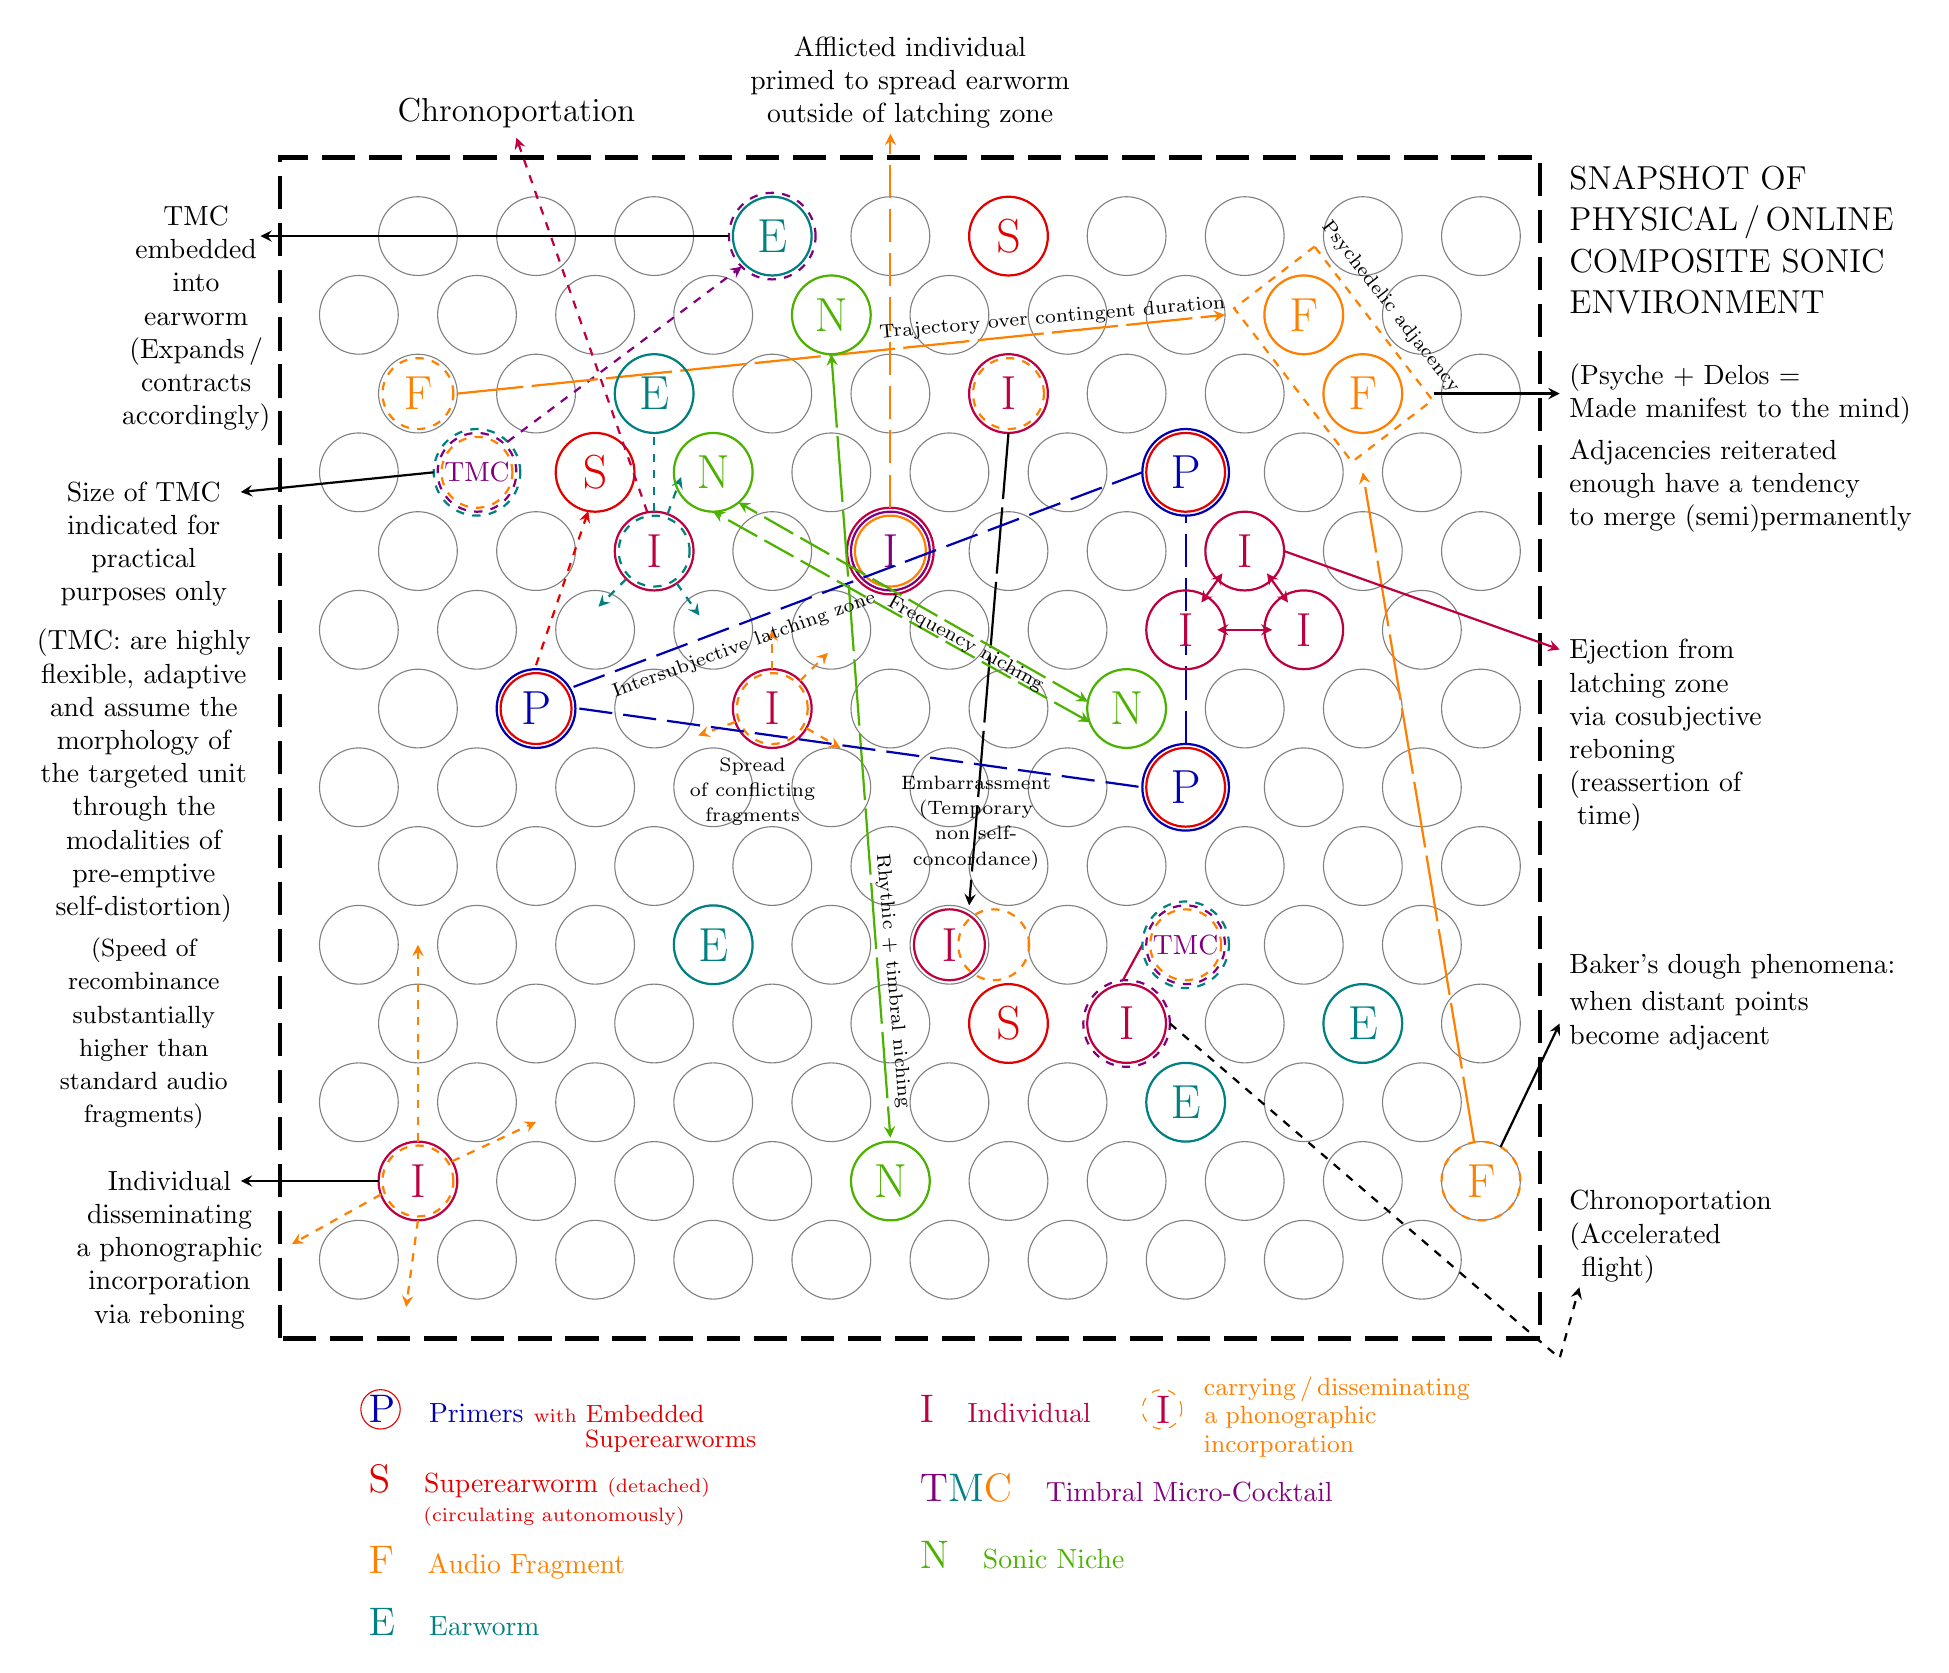
\begin{tikzpicture}	
	%MAIN CIRCLEs
	\draw[ultra thick,dashed,dash pattern=on 12pt off 5pt] (0,0) rectangle (16,15);
	\foreach \i in {0,...,9}{
	\foreach \j in {0,...,6}{
		\draw[gray] (1+1.5*\i,1+2*\j) circle (0.5cm);
		\draw[gray] (1.75+1.5*\i,2+2*\j) circle (0.5cm);
	} %end j loop
	} %end i loop
	
	%COLORED CIRCLES
	\draw[purple,thick] (1.75+1.5*0,2+2*0) circle (0.5cm) node {\LARGE I};
	\draw[orange,thick,dashed] (1.75+1.5*0,2+2*0) circle (0.45cm);
	\draw[thick,->,>=stealth] ({1.75+1.5*0+0.5*cos(180)},{2+2*0+0.5*sin(180)})--(-0.5,2);
	\draw[thick,->,>=stealth,orange,dashed] ({1.75+1.5*0+0.5*cos(200)},{2+2*0+0.5*sin(200)})--(0.15,1.2);
	\draw[thick,->,>=stealth,orange,dashed] ({1.75+1.5*0+0.5*cos(270)},{2+2*0+0.5*sin(270)})--(1.6,0.4);
	\draw[thick,->,>=stealth,orange,dashed] ({1.75+1.5*0+0.5*cos(90)},{2+2*0+0.5*sin(90)})--(1.75,5);
	\draw[thick,->,>=stealth,orange,dashed] ({1.75+1.5*0+0.5*cos(30)},{2+2*0+0.5*sin(30)})--(3.25,2.75);
	
	%needs to be before 'trajectory' caption
	\draw[violet,thick] (1.75+1.5*4,2+2*4) circle (0.5cm) node {\LARGE I};
	\draw[purple,thick] (1.75+1.5*4,2+2*4) circle (0.55cm);
	\draw[orange,thick] (1.75+1.5*4,2+2*4) circle (0.45cm);
	\draw[orange,thick,->,>=stealth,dash pattern=on 12pt off 4pt] ({1.75+1.5*4+0.55*cos(90)},{2+2*4+0.55*sin(90)}) -- ++(0,4.75);
	
	\draw[teal,thick] (1+1.5*3,1+2*2) circle (0.5cm) node {\LARGE E};
	\draw[blue!70!black,thick] (1.75+1.5*1,2+2*3) circle (0.5cm) node {\LARGE P};
		\draw[thick,->,>=stealth,red!90!black,dashed] ({1.75+1.5*1+0.55*cos(90)},{2+2*3+0.55*sin(90)})-- ({1+1.5*2+0.5*cos(260)},{1+2*5+0.5*sin(260)});
	\draw[red!90!black,thick] (1.75+1.5*1,2+2*3) circle (0.45cm);
	\draw[red!90!black,thick] (1+1.5*2,1+2*5) circle (0.5cm) node {\LARGE S};
	%
	\draw[white,thick] (1+1.5*1,1+2*5) circle (0.5cm); %cover up gray
	\draw[violet,thick,dashed] (1+1.5*1,1+2*5) circle (0.5cm) node {TMC};
	\draw[orange,thick,dashed] (1+1.5*1,1+2*5) circle (0.45cm);
	\draw[teal,thick,dashed] (1+1.5*1,1+2*5) circle (0.55cm);
	\draw[violet,thick,->,>=stealth,dashed] ({1+1.5*1+0.55*cos(45)},{1+2*5+0.55*sin(45)}) -- ({1.75+1.5*3+0.55*cos(225)},{2+2*6+0.55*sin(225)});
	\draw[thick,->,>=stealth] ({1+1.5*1+0.55*cos(180)},{1+2*5+0.55*sin(180)}) -- (-0.5,10.75);
	%
	\draw[orange,thick,dashed] (1.75+1.5*0,2+2*5) circle (0.45cm) node {\LARGE F};
	\draw[orange,thick,->,>=stealth,dash pattern=on 24pt off 3pt] ({1.75+1.5*0+0.5*cos(0)},{2+2*5+0.5*sin(0)}) -- (12,13) node[pos=0.775,black,above,yshift=-0.25cm]{\rotatebox{5}{\scriptsize Trajectory over contingent duration}};
	
	\draw[teal,thick] (1.75+1.5*2,2+2*5) circle (0.5cm) node {\LARGE E};
	\draw[purple,thick] (1.75+1.5*2,2+2*4) circle (0.5cm) node {\LARGE I};
	\draw[teal,thick,dashed] (1.75+1.5*2,2+2*4) circle (0.45cm);
	\draw[teal,thick,dashed] ({1.75+1.5*2+0.5*cos(90)},{2+2*4+0.5*sin(90)}) -- ({1.75+1.5*2+0.5*cos(270)},{2+2*5+0.5*sin(270)});
	\draw[teal,thick,dashed,->,>=stealth] ({1.75+1.5*2+0.5*cos(70)},{2+2*4+0.5*sin(70)}) -- ({1.75+1.5*2+1*cos(70)},{2+2*4+1*sin(70)});
	\draw[teal,thick,dashed,->,>=stealth] ({1.75+1.5*2+0.5*cos(225)},{2+2*4+0.5*sin(225)}) -- ({1.75+1.5*2+1*cos(225)},{2+2*4+1*sin(225)});
	\draw[teal,thick,dashed,->,>=stealth] ({1.75+1.5*2+0.5*cos(305)},{2+2*4+0.5*sin(305)}) -- ({1.75+1.5*2+1*cos(305)},{2+2*4+1*sin(305)});
	\draw[purple,thick,dashed,->,>=stealth] ({1.75+1.5*2+0.5*cos(100)},{2+2*4+0.5*sin(100)}) -- (3,15.25);
	
	\draw[purple,thick] (1.75+1.5*3,2+2*3) circle (0.5cm) node {\LARGE I};
	\draw[orange,thick,dashed] (1.75+1.5*3,2+2*3) circle (0.45cm);
	\draw[orange,thick,->,>=stealth,dashed] ({1.75+1.5*3+0.5*cos(45)},{2+2*3+0.5*sin(45)}) -- ({1.75+1.5*3+1*cos(45)},{2+2*3+1*sin(45)});
	\draw[orange,thick,->,>=stealth,dashed] ({1.75+1.5*3+0.5*cos(90)},{2+2*3+0.5*sin(90)}) -- ({1.75+1.5*3+1*cos(90)},{2+2*3+1*sin(90)});
	\draw[orange,thick,->,>=stealth,dashed] ({1.75+1.5*3+0.5*cos(200)},{2+2*3+0.5*sin(200)}) -- ({1.75+1.5*3+1*cos(200)},{2+2*3+1*sin(200)});
	\draw[orange,thick,->,>=stealth,dashed] ({1.75+1.5*3+0.5*cos(-30)},{2+2*3+0.5*sin(-30)}) -- ({1.75+1.5*3+1*cos(-30)},{2+2*3+1*sin(-30)});
	\node[align=center,below] at (6,7.5) {%
		\scriptsize Spread \\[-1mm] \scriptsize of conflicting \\[-1mm] \scriptsize fragments
	};
	
	\draw[red!90!black,thick] (1.75+1.5*5,2+2*6) circle (0.5cm) node {\LARGE S};
	
	\draw[green!40!olive,thick] (1+1.5*3,1+2*5) circle (0.5cm) node {\LARGE N};
	\draw[green!40!olive,thick] (1+1.5*4,1+2*6) circle (0.5cm) node {\LARGE N};
	
	\draw[teal,thick] (1.75+1.5*3,2+2*6) circle (0.5cm) node {\LARGE E};
	\draw[violet,thick,dashed] (1.75+1.5*3,2+2*6) circle (0.55cm);
	\draw[thick,->,>=stealth] ({1.75+1.5*3+0.55*cos(180)},{2+2*6+0.55*sin(180)})--(-0.25,14);
	
	\draw[green!40!olive,thick] (1.75+1.5*4,2+2*0) circle (0.5cm) node {\LARGE N};
	\draw[green!40!olive,thick,<->,>=stealth,dash pattern=on 24pt off 3pt] ({1+1.5*4+0.5*cos(270)},{1+2*6+0.5*sin(270)}) -- ({1.75+1.5*4+0.55*cos(90)},{2+2*0+0.55*sin(90)}) node[pos=0.8,black,right,xshift=-0.2cm]{\rotatebox{-85}{\scriptsize Rhythic + timbral niching}};
	
	\draw[purple,thick] (1+1.5*5,1+2*2) circle (0.45cm) node {\LARGE I};
	\draw[orange,thick,dashed] (1+1.5*5.375,1+2*2) circle (0.45cm);
	
	\draw[red!90!black,thick] (1.75+1.5*5,2+2*1) circle (0.5cm) node {\LARGE S};
	\draw[purple,thick] (1.75+1.5*6,2+2*1) circle (0.5cm) node {\LARGE I};
	\draw[violet,thick,dashed] (1.75+1.5*6,2+2*1) circle (0.55cm);
	\draw[teal,thick] (1+1.5*7,1+2*1) circle (0.5cm) node {\LARGE E};
	%
	\draw[purple,thick] ({1.75+1.5*6+0.55*cos(95)},{2+2*1+0.55*sin(95)}) -- ({1+1.5*7+0.55*cos(180)},{1+2*2+0.55*sin(180)}); %TMC--I
	\draw[thick,->,>=stealth,dashed] ({1.75+1.5*6+0.55*cos(0)},{2+2*1+0.55*sin(0)}) -- (16.25,-0.25) -- (16.5,0.65);
	%
	\draw[white,thick] (1+1.5*7,1+2*2) circle (0.5cm); %cover up gray
	\draw[violet,thick,dashed] (1+1.5*7,1+2*2) circle (0.5cm) node {TMC};
	\draw[orange,thick,dashed] (1+1.5*7,1+2*2) circle (0.45cm);
	\draw[teal,thick,dashed] (1+1.5*7,1+2*2) circle (0.55cm);
	
	\draw[purple,thick] (1.75+1.5*5,2+2*5) circle (0.5cm) node {\LARGE I};
	\draw[orange,thick,dashed] (1.75+1.5*5,2+2*5) circle (0.45cm);
	\draw[thick,->,>=stealth,dash pattern=on 24pt off 3pt] ({1.75+1.5*5+0.5*cos(270)},{2+2*5+0.5*sin(270)}) -- (8.75,5.5) node[pos=0.825,black,align=center]{%
		\scriptsize Embarrassment \\[-1mm]
		\scriptsize (Temporary \\[-1mm]
		\scriptsize non self- \\[-1mm]
		\scriptsize concordance)
	};
	
	\draw[red!90!black,thick] (1+1.5*7,1+2*3) circle (0.5cm);
	\draw[blue!70!black,thick] (1+1.5*7,1+2*3) circle (0.55cm) node {\LARGE P};
	\draw[red!90!black,thick] (1+1.5*7,1+2*5) circle (0.5cm);
	\draw[blue!70!black,thick] (1+1.5*7,1+2*5) circle (0.55cm) node {\LARGE P};
	\draw[blue!70!black,thick,dash pattern=on 12pt off 4pt] ({1+1.5*7+0.55*cos(90)},{1+2*3+0.55*sin(90)})--({1+1.5*7+0.55*cos(270)},{1+2*5+0.55*sin(270)});
	\draw[blue!70!black,thick,dash pattern=on 12pt off 4pt] ({1.75+1.5*1+0.55*cos(30)},{2+2*3+0.55*sin(30)})--({1+1.5*7+0.55*cos(180)},{1+2*5+0.55*sin(180)}) node[pos=0.3,black,below,yshift=0.55cm]{\rotatebox{20}{\scriptsize Intersubjective latching zone}};
	\draw[blue!70!black,thick,dash pattern=on 12pt off 4pt] ({1.75+1.5*1+0.55*cos(0)},{2+2*3+0.55*sin(0)})--({1+1.5*7+0.55*cos(180)},{1+2*3+0.55*sin(180)});
	
	\draw[orange,thick,dashed] (1.75+1.5*9,2+2*0) circle (0.5cm) node {\LARGE F};
	\draw[teal,thick] (1.75+1.5*8,2+2*1) circle (0.5cm) node {\LARGE E};
	\draw[orange,thick] (1.75+1.5*8,2+2*5) circle (0.5cm) node {\LARGE F};
	\draw[orange,thick] (1+1.5*8,1+2*6) circle (0.5cm) node {\LARGE F};
	\node[rectangle,draw=orange,rotate=37.5,yscale=10.5,xscale=5.5,thick,dashed] at (1.375+1.5*8,1.5+2*5.5) {};
	\node at (14.1,13.1) {\rotatebox{-52}{\scriptsize Psychedelic adjacency}};
	\draw[orange,thick,->,>=stealth,dash pattern=on 24pt off 3pt] ({1.75+1.5*9+0.5*cos(100)},{2+2*0+0.5*sin(100)}) -- (13.75,11);
	\draw[thick,->,>=stealth] ({1.75+1.5*9+0.5*cos(60)},{2+2*0+0.5*sin(60)}) -- (16.25,4);
	\draw[thick,->,>=stealth] (14.65,12)--(16.25,12);
	
	\draw[purple,thick] (1+1.5*7,1+2*4) circle (0.5cm) node {\LARGE I};
	\draw[purple,thick] (1+1.5*8,1+2*4) circle (0.5cm) node {\LARGE I};
	\draw[purple,thick] (1.75+1.5*7,2+2*4) circle (0.5cm) node {\LARGE I};
	\draw[purple,thick,<->,>=stealth] ({1.75+1.5*7+0.4*cos(225)},{2+2*4+0.4*sin(225)}) -- ({1+1.5*7+0.4*cos(60)},{1+2*4+0.4*sin(60)});
	\draw[purple,thick,<->,>=stealth] ({1.75+1.5*7+0.4*cos(-45)},{2+2*4+0.4*sin(-45)}) -- ({1+1.5*8+0.4*cos(120)},{1+2*4+0.4*sin(120)});
	\draw[purple,thick,<->,>=stealth] ({1+1.5*7+0.4*cos(0)},{1+2*4+0.4*sin(0)}) -- ({1+1.5*8+0.4*cos(180)},{1+2*4+0.4*sin(180)});
	\draw[purple,thick,->,>=stealth] ({1.75+1.5*7+0.5*cos(0)},{2+2*4+0.5*sin(0)}) -- (16.25,8.75);
	
	\draw[green!40!olive,thick] (1.75+1.5*6,2+2*3) circle (0.5cm) node {\LARGE N};
	\draw[green!40!olive,thick,<->,>=stealth,dash pattern=on 12pt off 3pt] ({1.75+1.5*6+0.5*cos(200)},{2+2*3+0.5*sin(200)}) -- ({1+1.5*3+0.5*cos(270)},{1+2*5+0.5*sin(270)});
	\draw[green!40!olive,thick,<->,>=stealth,dash pattern=on 12pt off 3pt] ({1.75+1.5*6+0.5*cos(170)},{2+2*3+0.5*sin(170)}) -- ({1+1.5*3+0.5*cos(310)},{1+2*5+0.5*sin(310)}) node[pos=0.35,black,yshift=-0.15cm] {\rotatebox{-29}{\scriptsize Frequency niching}};
	
%------------------------------------------------------------------------------------
	
	%OUTER LABELS
	\node[above] at (3,15.25) {\large Chronoportation};
	\node[above,align=center] at (8,15.25) {%
		 Afflicted individual \\ primed to spread earworm \\ outside of latching zone
	};
	
	\node[align=center,below left] at (0,14.5) {%
	 TMC \\ embedded \\ into \\ earworm \\%
	 (Expands$\,$/ \\ contracts \\ accordingly)
	};
	\node[align=center,below left] at (-0.25,11) {%
		 Size of TMC \\ indicated for \\ practical \\ purposes only \\[2mm]%
		 (TMC: are highly \\ flexible, adaptive \\ and assume the \\ morphology of \\ the targeted unit \\ through the \\ modalities of \\ pre-emptive \\ self-distortion) \\[1mm]%
		 \small (Speed of \\\small recombinance \\\small substantially \\\small higher than \\\small standard audio \\\small fragments)
	};
	\node[align=center,below left] at (-0.1,2.25) {%
		 Individual \\ disseminating \\ a phonographic \\ incorporation \\ via reboning
	};
	
	\node[align=left,below right] at (16.25,15) {%
		\large SNAPSHOT OF \\[1mm]\large  PHYSICAL$\,$/$\,$ONLINE \\[1mm]\large COMPOSITE SONIC \\[1mm]\large  ENVIRONMENT
	};
	\node[align=left,below right] at (16.25,12.5) {%
		(Psyche + Delos = \\ Made manifest to the mind) \\[1mm] Adjacencies reiterated \\ enough have a tendency \\ to merge (semi)permanently
	};
	\node[align=left,below right] at (16.25,9) {%
		 Ejection from \\ latching zone \\ via cosubjective \\ reboning \\ (reassertion of \\ $\;$time)
	};
	\node[align=left,below right] at (16.25,5) {%
		Baker's dough phenomena: \\[0.5mm] when distant points \\ become adjacent
	};
	\node[align=left,below right] at (16.25,2) {%
		Chronoportation \\ (Accelerated \\ $\;\,$flight)
	};
	
%------------------------------------------------------------------------------------
	
	%BOTTOM LEGEND
	\node[blue!70!black,align=left,right] at (1,-0.9) {{\Large P} $\;\;$ Primers};
	\node[red!90!black,align=left,right] at (3,-1.15) {$\;$%
		{\scriptsize with} 
		{\small Embedded} \\[-1mm]\hspace{0.75cm}\small Superearworms};
	\draw[red!90!black] (1.275,-0.9) circle (0.25cm);
	\node[red!90!black,align=left,right] at (1,-2) {{\Large S} $\;\;$ 
		Superearworm {\scriptsize (detached)}\\[-0.5mm]
		\scriptsize\hspace{0.6cm} (circulating autonomously)
	};
	\node[orange,align=left,right] at (1,-2.85) {{\Large F} $\;\;$ Audio Fragment};
	\node[teal,align=left,right] at (1,-3.6) {{\Large E} $\;\;$ Earworm};
	
	\node[purple,align=left,right] at (8,-0.9) {{\Large I} $\;\;$ Individual};
	\node[violet,align=left,right] at (8,-1.9) {{\Large T{\color{teal}M}{\color{orange}C}} $\;\;$ Timbral Micro-Cocktail};
	\node[green!40!olive,align=left,right] at (8,-2.75) {{\Large N} $\;\;$ Sonic Niche};
	\node[orange,align=left,right] at (11,-1) {%
		\small\hspace{0.5cm} carrying$\,$/$\,$disseminating \\[-1mm]
		{\Large\color{purple} I}\small $\;\;\;\,$ a phonographic \\[-0.5mm]
		\small\hspace{0.5cm} incorporation
	};
	\draw[orange,dashed] (11.2,-0.9) circle (0.25cm);
	
	%\draw[help lines] (0,0) grid (16,15);
	\end{tikzpicture}
	
\end{document}